\documentclass[11pt]{article}
\usepackage[margin=1in]{geometry}
\usepackage[T1]{fontenc}
\usepackage{lmodern,amsmath,amssymb,amsthm,booktabs,graphicx,longtable,array}
\usepackage[colorlinks=true,allcolors=blue]{hyperref}
\usepackage{microtype}
\newtheorem{proposition}{Proposition}
\newtheorem{corollary}{Corollary}
\newcommand{\ind}{\mathbf{1}}
\title{The Order of Transformation:\\Learning, Remediation, and the Option to Stop}
\author{Dr. Jan-Hendrik Weinert}
\date{19 October 2026}

% Publication formatting edition, 19 October 2026. Scientific equations unchanged.
\usepackage{xurl,needspace,etoolbox}
\geometry{a4paper,margin=25.4mm}
\hypersetup{hidelinks,pdfauthor={Dr. Jan-Hendrik Weinert}}
\setlength{\parindent}{1.2em}
\setlength{\parskip}{3pt plus 1pt}
\setlength{\emergencystretch}{3em}
\raggedbottom
\pagestyle{plain}
\makeatletter
\renewcommand{\@seccntformat}[1]{\csname the#1\endcsname\ifstrequal{#1}{section}{.}{}\quad}
\renewcommand{\maketitle}{%
  \begin{center}
  {\LARGE\bfseries\@title\par}
  \vspace{0.8em}
  {\normalsize\@author\par}
  \vspace{0.35em}
  {\small\@date\par}
  \end{center}
  \vspace{0.4em}}
\renewenvironment{abstract}{%
  \begin{center}\small\bfseries Abstract\end{center}
  \begin{list}{}{\setlength{\leftmargin}{0.5in}\setlength{\rightmargin}{0.5in}}
  \item[]\small\setlength{\parindent}{0pt}\ignorespaces
}{\end{list}\vspace{0.6em}}
\makeatother

\begin{document}
\maketitle
\begin{abstract}
Implementation order trades off better diagnosis against the option to avoid sunk remediation costs. We solve a binary learning and entry-certificate model with endogenous production experimentation, direct remediation and no remediation. Under the stated information ordering and equal assigned pilot costs, tools-first dominates all alternatives exactly on an open physical-cost interval. Closed-form cutoffs identify its competitors and the pilot-cost ceiling for nonemptiness. Synthetic primitives yield the full certificate-fee partition, all ties and an explicit reset threshold at which the interval disappears. Known repair, an independent reset and revealing public validation retain their Bayesian nulls. The contribution is a model-specific cost and fee characterization, supported by complete proofs and executable checks; no firm data are analyzed.
\end{abstract}
\noindent\small \noindent\textbf{Keywords:} implementation order; Bayesian experimentation; credible validation; irreversible remediation; organizational transformation.
\par \textbf{JEL:} D83, L23, O32, C93.\par\normalsize
\vspace{0.6em}
\section{Introduction}
Two organizations may install the same data remediation and decision-support components yet use them differently. A familiar explanation is that an early failure destroys trust. That explanation is incomplete unless it states what the failure reveals about the repaired system and why users do not acquire better evidence. We study those questions in a small rational model and use the original adaptive-willingness model only as a behavioral benchmark.

Our starting distinction is between physical installation and information about effectiveness. A remediation can be visible while its persistent residual effectiveness is uncertain. Early outcomes then matter only to the extent that they predict that residual component under the correct likelihood. A known complete reset erases their predictive content. A credible public validation can also resolve it; a managerial assurance that physical work occurred need not do so. This distinction permits rational non-use after an unlucky history without treating correct Bayesian conditioning as a bias.

We solve a two-task user problem with a safe outside option, endogenous use-based experimentation, and a costly fully revealing entry validation. A closed-form experimentation boundary and a piecewise-affine value function characterize every posterior. A separate sufficient-condition result shows when indefinite abstention is optimal even with an infinite horizon. Neither result is offered as a new theory of bandit stopping. They discipline the sequencing question and expose an impossibility: at fixed final technology, timing, costs and action opportunities, free additional correctly interpreted information cannot reduce ex-ante optimized value. The earlier tools-first engagement example relied on unequal exposure and does not survive an equal-count benchmark in the claimed form.

The primary policy result compares one diagnostic before remediation with one after it, with common production dates and equal diagnostic cost. A pre-remediation signal may be noisier, but it arrives before an avoidable physical expenditure. We solve the menu of no remediation, direct remediation, tools-first with contingent abandonment, and foundations-first with sunk remediation, each allowing an optimal validation purchase. The exact difference between the ordered policies is the value of screening out unnecessary remediation minus the continuation value of better diagnosis, plus any explicitly unequal diagnostic costs. Under a stated information ordering, forcing both policies to complete remediation removes the screening term and weakly favors the more informative post-remediation diagnostic. Thus the reason tools-first can be efficient is a real option to stop, not presumed psychological primacy.

Solved synthetic examples exhibit foundations-first, tools-first, direct repair with cheap verification, and no repair as respective optima. Exhaustive two-task policy enumeration and independent numerical checks verify the formulas. A generic repeated-team carryover simulation and an unrun field protocol are retained separately in the appendices. They neither estimate the model nor validate structural trust. There are no firm data or completed experiments.

The contribution is the exact cost-region characterization in Propositions~\ref{prop:window} and \ref{prop:resetregion}, rather than the screening decomposition. With equal assigned pilot costs we derive necessary and sufficient bounds against all three alternatives, solve the certificate-fee breakpoints for the declared baseline, and characterize when reset makes the strict region empty. Direct entry and no repair materially constrain the region: an ordered-policy advantage alone does not imply an optimal pilot. The full weak partition retains zero-cost tails and all equality faces. The result is a small model-specific analytic decision certificate, not a new general theorem about the value of information, investment options or selective non-learning.

\section{Closest literature and the boundary of the contribution}
Jovanovic and Stolyarov's \emph{Optimal Adoption of Complementary Technologies} (2000) is the closest dynamic complementary-investment comparator. The published record and an indexed mathematical passage from the author-hosted final article were verified: its objective includes flow production $\min\{x,z\}$ and the costs of discrete upgrades. Nonconvex adjustment costs can induce asynchronous adoption. Our expenditure-order question is related, but the decision object here is a diagnostic experiment followed by optional remediation and verification; the frontier separates information quality from avoided sunk spending. We do not claim the fixed-cost or asynchronous-adoption insight. The scanned final article could not be fully extracted; the comparison is grounded in its verified objective and argument, not an exhaustive theorem exclusion.

Their \emph{Learning, Complementarities, and Asynchronous Use of Technology} is separately verified as NBER Working Paper 5870, January 1997. Its official abstract describes a learning period after an upgrade and asynchronous purchases to avoid underutilized complementary inputs. We keep that working-paper citation separate and do not assume it is an identical earlier version of the 2000 final article. Formaneck and Cozzarin (2013), verified at abstract level, already optimize budget-constrained paths through technology and training choices. Neither asynchronous implementation nor optimal paths are new claims here.

Repenning and Sterman (2002) develop an empirically motivated process-improvement model in which delayed benefits and mutually reinforcing attributions can sustain failure to improve. The published citation is \emph{Administrative Science Quarterly} 47(2):265--295. Its author-hosted forthcoming description was read; MIT's separate working-paper record 4372-02 has a repository issue date in 2003. A repository date is not a different publication year for the journal article. The working-paper download was blocked, so we do not equate every working-model equation with its final version. Our rational benchmark imposes no attribution bias: beliefs use correct pre/post likelihoods, stopping is optimal, and common-information welfare is aligned. The cost-region theorem below, rather than the inherited screening decomposition, is the decision-specific comparison beyond a capability-trap narrative.

Bayesian experimentation already permits optimal cessation of informative actions. Rothschild's (1974) market-pricing paper is a classical precedent; its final bibliography was verified, but inaccessible full text prevents detailed theorem attribution. Fudenberg and Levine's (1993) final \emph{Self-Confirming Equilibrium}, retrieved in indexed primary passages including pp. 523--524, explicitly separates on-path evidence from unobserved alternatives and discusses incentives to experiment. Our single-user stopping model is not a new strategic equilibrium concept, and a mistaken realized belief under a correct prior is not automatically an instance of their equilibrium. Bergemann and V\"alim\"aki's (2006) \emph{Bandit Problems} is cited as a verified Cowles discussion paper, not as the scanned later reprint encountered in retrieval. The exploration/exploitation problem and endogenous non-learning are background, not discoveries.

Blackwell (1953) supplies experiment comparison; positive-part accounting and the value of retaining an expenditure option are inherited. Epstein (1980), read in the author-hosted final article, is a closer primary comparator than complementary-capital adoption alone. His equation (1) is a preposterior optimization over a first decision and a posterior-contingent second decision. Section 3, p.~275 explicitly permits binary actions: commitment removes subsequent flexibility, and better future information discourages irreversible commitment. Map the uncertain state to final quality, the message to the diagnostic, and continuation payoff to optimized production. This directly supplies our qualitative screening logic. It does not evaluate our four-policy menu's certificate-fee cells or its two lower cost cutoffs; these require inserting the entry-certificate and two-task continuation values. We solve that adjacent concrete decision margin in Section~\ref{sec:regions}, while claiming no new general irreversibility principle. The same article's smooth comparative-static theorem in Section 2 is distinct from its binary Section 3 argument; discrete actions do not evade that predecessor.

Xu, Zariphopoulou and Zhang's \emph{Decision Making under Costly Sequential Information Acquisition} is read as arXiv:2401.00569v4, revised 6 January 2026, not as a verified final journal article. Its Section 2, equations (2.1)--(2.10), studies costly Gaussian learning followed by a choice whose reward can itself solve a subsequent information problem; Section 2.1 allows finer information after choosing the uncertain product and costly return. Thus nested information regimes and subsequent learning are already explicit primary-literature objects. Their stopping-time and return-fee decisions differ from our fixed assigned binary pilot, optional physical outlay, and entry-only perfect certificate. Our exact finite fee/cost partition is not claimed to supersede their richer model. No located predecessor was found to state this particular partition; that bounded access result is not a proof of global originality. Failed downloads are recorded as access limitations, never evidence that a theorem is absent.

Vahter and Vadi (2024) are the closest verified empirical sequence comparison. Their accessible 2022 working version analyzes innovation transitions rather than randomized remediation and support. We distinguish that detailed working-version reading from verified final publication metadata. Brynjolfsson, Rock and Syverson (2021) explain complementary intangibles and productivity measurement, not our diagnosis/stopping frontier; their 2018 working version and final publication are separately identified. Dietvorst et al. (2015), Kawaguchi (2021), Desai et al. (2012) and Syharat et al. (2026) motivate behavioral and operational measurement, not the rational propositions. Murphy (2005) informs the proposed randomized-strategy protocol. None supplies firm-level evidence for this model, and no universal timing effect is presumed.

\section{Rational learning after physical remediation}\label{sec:rational}
\subsection{What is known, and what a repair does not reveal}
There are two persistent potential types of the completed workflow, $\theta_1\in\{H,L\}$. Conditional on the type, an operational recommendation succeeds with probability $b_H$ or $b_L$, independently over tasks. A success pays one, a failure pays zero, and each use costs $c$, where
\[
 0<b_L<c<b_H<1,\qquad m(p)=b_L+(b_H-b_L)p-c.
\]
The safe manual decision has incremental payoff zero and reveals nothing about the tool. Physical remediation costs $K\geq0$. It installs the same technical component under either sequence; without it, production remains manual. A pre-remediation shadow pilot is possible but has no operating payoff. This separates diagnostic experience from actual production and makes ``no remediation'' a well-defined feasible policy. The planner and user are risk neutral, have the same payoff and prior, and observe every pilot, implementation action, and certificate. There is no hidden planner information, transfer motive, or assumed irrational distrust.

To specify uncertain effectiveness and persistence, let $\theta_0$ be the pre-remediation type with prior $\Pr(H)=p_0\in(0,1)$. A pre-remediation pilot succeeds with known probabilities $a_H>a_L$ conditional on $\theta_0$. Following physical remediation, with known probability $1-\zeta$ the persistent type remains $\theta_0$; with probability $\zeta$ it is independently redrawn from the original prior $p_0$. The realized redraw and resulting effectiveness are not directly observed. The completed system then retains $\theta_1$ over the production horizon. Its unconditional prior is still $p_0$. The parameters $(a_H,a_L,b_H,b_L,c,\zeta,K)$ and conditional independence structure are common knowledge. In particular, users know the difference between pre- and post-remediation performance; they never use the old likelihood to interpret a new observation.

For an early history $h$ with posterior $q(h)=\Pr(\theta_0=H\mid h)$, correct conditioning on observed physical installation gives
\begin{equation}
 p(h)=\Pr(\theta_1=H\mid h,F)=\zeta p_0+(1-\zeta)q(h).\label{eq:reset}
\end{equation}
Thus $q_0$ and $q_1$ are not known realized performance levels in this model. Their counterparts are the known conditional success probabilities $a_{\theta_0}$ and $b_{\theta_1}$; the types are unknown. Remediation can change average quality without making its realized effectiveness public. No assumption says every realization of remediation improves every type; the numerical baseline $\zeta=0$ does have $a_H<b_H$ and $a_L<b_L$.

For a single early pilot, define $\bar a=p_0a_H+(1-p_0)a_L$. As an experiment about the \emph{final} type, its effective likelihoods are
\begin{equation}
 A_H=(1-\zeta)a_H+\zeta\bar a,\qquad
 A_L=(1-\zeta)a_L+\zeta\bar a.\label{eq:effective}
\end{equation}
They follow by summing over the joint old/final type distribution. Explicitly,
\[
\begin{array}{c|cc}
 &\theta_1=H&\theta_1=L\\\hline
\theta_0=H&p_0(1-\zeta+\zeta p_0)&\zeta p_0(1-p_0)\\
\theta_0=L&\zeta p_0(1-p_0)&(1-p_0)(1-\zeta+\zeta(1-p_0)).
\end{array}
\]
Dividing the first column's signal-weighted entries by its marginal $p_0$ gives $A_H$, and dividing the second by $1-p_0$ gives $A_L$. Summing over a history before the redraw gives (\ref{eq:reset}) by the law of total probability. Bayes' rule with these likelihoods gives exactly (\ref{eq:reset}). At $\zeta=1$, the early signal is uninformative about the final system, even though it may have been informative about the old one. ``A repair was installed'' and ``the repaired workflow is effective'' are distinct observations.

\subsection{Endogenous experimentation: an exact two-task solution}\label{sec:bellman}
There are two production opportunities, at common calendar dates 2 and 3, with discount factor $\delta\in(0,1)$. At each opportunity the user chooses the safe decision or use. An observed success or failure updates the final-type posterior. Define the predictive success probability $\bar b(p)=pb_H+(1-p)b_L$ and the Bayesian updates
\begin{equation}
 p^+=\frac{pb_H}{\bar b(p)},\qquad
 p^-=\frac{p(1-b_H)}{1-\bar b(p)}.\label{eq:bayes}
\end{equation}
The one-task value is $V_1(p)=[m(p)]_+$, with $[x]_+=\max(x,0)$. Without an external certificate, the two-task value is
\begin{equation}
 V_2(p)=\left[m(p)+\delta\{\bar b(p)V_1(p^+)+(1-\bar b(p))V_1(p^-)\}\right]_+.\label{eq:v2}
\end{equation}
The maximization here is over a real information-producing action, not an imposed willingness threshold. Choosing safe now and using later has value $\delta[m(p)]_+$ and is weakly dominated: when $m(p)>0$, use now yields at least $(1+\delta)m(p)$ by Jensen's inequality; when $m(p)\leq0$, safe-now/safe-later gives zero. The finite horizon is explicit, not evidence of infinite persistence.

\begin{proposition}[A Bayesian experimentation boundary]\label{prop:bayes}
Let $h=b_H-c>0$, $\ell=b_L-c<0$, $\Delta=b_H-b_L$, and
\begin{align}
 S&=\Delta+\delta(b_Hh-b_L\ell),&
 p_*&=\frac{-\ell(1+\delta b_L)}{S},\\
 t_-&=\frac{-(1-b_L)\ell}{(1-b_H)h-(1-b_L)\ell}.
\end{align}
Then $0<p_*< (c-b_L)/\Delta<t_-<1$, and the exact solution is
\begin{equation}
 V_2(p)=\begin{cases}
 0,&0\leq p\leq p_*,\\
 \ell(1+\delta b_L)+Sp,&p_*<p<t_-,\\
 (1+\delta)(\ell+\Delta p),&t_-\leq p\leq1.
 \end{cases}\label{eq:piecewise}
\end{equation}
Except at ties, users abstain at the first opportunity if $p<p_*$ and experiment if $p>p_*$. In particular, some negative-current-return experiments are optimal because they can improve the last decision.
\end{proposition}
\begin{proof}
Multiplying terminal payoffs by their predictive probabilities removes the Bayes denominators. The continuation term is
\[
 [pb_Hh+(1-p)b_L\ell]_+
 +[p(1-b_H)h+(1-p)(1-b_L)\ell]_+.
\]
Both bracketed affine expressions increase strictly in $p$. Their zeroes are $t_+=-b_L\ell/(b_Hh-b_L\ell)$ and $t_-$, respectively. At the myopic zero $t_0=-\ell/\Delta$, a success raises the posterior above $t_0$ and a failure lowers it, so $0<t_+<t_0<t_-<1$. The untruncated use value $Q_2$ is continuous and strictly increasing. At $t_+$ its continuation terms are zero and $m(t_+)<0$; at $t_0$, its success continuation term is strictly positive. Its unique zero is therefore in $(t_+,t_0)$, where only the success continuation term is positive. Solving the affine equation there gives $p_*$. Below it, use and any delayed use are dominated by zero. Between $p_*$ and $t_-$ only success leads to terminal use. Above $t_-$, both outcomes lead to terminal use, and the martingale property of posterior means gives $Q_2=(1+\delta)m(p)$. These arguments give every branch and the boundary inequalities.
\end{proof}

\subsection{Costly credible validation and rational non-use}\label{sec:certificate}
After physical remediation and any assigned pilot, but before date 2, a user can buy a credible independent certificate for fee $k\geq0$. The certificate perfectly reveals $\theta_1$ and is publicly and mandatorily disclosed, including unfavorable results. Its fee is a real verification cost, not a transfer. It is available only in this entry window: its operational turnaround after date 2 would exceed the remaining task, so a mid-horizon purchase is not in the feasible menu. This restriction matters; an additional later validation option would change (\ref{eq:v2}) and is not silently included. Both sequences have exactly the same entry option. The planner can fund it, but with aligned payoffs funding does not alter its optimal purchase rule.

Given $H$, optimal use at both dates yields $B=(1+\delta)(b_H-c)$; given $L$, safe decisions yield zero. Thus the optimal entry value, including endogenous validation, is
\begin{equation}
 W(p;k)=\max\{V_2(p),pB-k\}.\label{eq:W}
\end{equation}
A self-reported managerial claim that remediation worked is not a certificate and supplies no extra signal under these information assumptions.

\begin{proposition}[Validation region and optimal abstention]\label{prop:validate}
The value of perfect information before its fee is $D(p)=pB-V_2(p)\geq0$. It is continuous, concave, and piecewise affine, with breakpoints among $0,p_*,t_-,1$ and endpoint values zero. A certificate is strictly preferred exactly where $D(p)>k$. This set is an interval or empty; its boundaries are obtained by solving the affine equations $D(p)=k$ on those pieces. Its maximal feasible fee is $\max\{D(p_*),D(t_-)\}$. Without purchase, private abstention is optimal exactly when $p\leq p_*$; with the entry option, abstention is optimal when both $p\leq p_*$ and $pB\leq k$.
\end{proposition}
\begin{proof}
For every fixed contingent two-task decision rule, its ex-ante expected payoff is affine in the prior. Their maximum $V_2$ is convex, also directly visible from (\ref{eq:piecewise}). Perfect information can reproduce any such rule after learning the type, so $pB\geq V_2(p)$. Subtracting a convex function from the affine $pB$ makes $D$ concave. Formula (\ref{eq:piecewise}) gives its breakpoints; a piecewise affine function achieves its maximum at one of its interior breakpoints or endpoints. The endpoints are zero. Comparing the two choices in (\ref{eq:W}) yields the purchase region. Finally $W=0$ if and only if both nonnegative outside-option value $V_2$ and certificate net value are nonpositive. At equality there can be indifferent nonzero actions; throughout we use safe decisions as the zero-value tie-break.
\end{proof}

A poor early outcome can therefore survive \emph{correctly understood} common physical remediation: it lowers $q(h)$ about a persistent component, (\ref{eq:reset}) leaves the final posterior low, and the user optimally rejects both risky experimentation and expensive certification. For example, take $(b_H,b_L,c,\delta)=(.9,.1,.5,.9)$, $p_0=.5$, $(a_H,a_L)=(.6,.08)$, $\zeta=0$ and $k=.35$. Then $p_*=.375862\ldots$. An early failure yields $p=.4/(.4+.92)=.303030\ldots$, so $V_2(p)=0$ and $pB-k<0$. Even when the realized final type happens to be $H$, abstention is optimal given the information. This is a false negative conditional on the realized type, not a violation of Bayesian rationality or an ex-ante welfare loss caused by information.

For completeness, a limited infinite-horizon statement shows that the logic need not rely solely on two tasks. Allow entry validation at any date at the same fee and let $A_\infty=(b_H-c)/(1-\delta)$. If
\begin{equation}
 m(p)+\delta pA_\infty\leq0,\qquad pA_\infty-k\leq0,\label{eq:infbound}
\end{equation}
then never using or validating is optimal, and beliefs remain unchanged forever in the absence of external observations. To prove this, any first use earns $m(p)$ and its continuation is bounded above by learning the type perfectly for free next period, with value $\delta pA_\infty$. Any first validation has net value at most $pA_\infty-k$. Safe waiting changes neither the posterior nor opportunities, so delaying either nonpositive first informative action cannot give positive value. This bounds all feasible policies, while perpetual safe play attains zero. These are sufficient conditions, not a solved general infinite-horizon cutoff. In the synthetic parameters above, three early failures give $p=.075947\ldots$, first-use upper bound about $-.0658$, and certification net value about $-.0462$ at $k=.35$. The event occurs with positive probability even for a truly effective type. The infinite-horizon certificate menu is explicitly larger than the entry-only two-task menu.

\section{When Bayesian conditioning rules out a sequence scar}\label{sec:impossibility}
\begin{proposition}[Reset, public evidence, and the value of extra information]\label{prop:impossible}
(i) If $\zeta=1$, histories before remediation do not change the posterior of final effectiveness. If successful repair instead makes the final success probability a publicly known $b>c$, all users use at both dates regardless of old outcomes. (ii) A fully revealing public certificate eliminates posterior differences about $\theta_1$: after a favorable certificate both histories induce use, and after an unfavorable one both induce safe decisions. (iii) With identical physical technology, costs, future opportunities and a common correctly specified prior, any free additional pre-decision experiment weakly increases ex-ante optimal continuation value. It cannot by itself create a negative expected ``trust scar.'' (iv) The order of a fixed set of conditionally independent signals about a fixed type is irrelevant at the common final decision date, provided signal identities and their correct likelihoods are retained and no earlier irreversible decisions differ.
\end{proposition}
\begin{proof}
For (i), set $\zeta=1$ in (\ref{eq:reset}); known $b$ leaves a positive known net payoff on each use. For (ii), posterior beliefs become 1 or 0, at which actions follow from $b_H>c>b_L$. For (iii), ignoring the extra experiment replicates the original feasible strategy. Equivalently, $W$ is convex as the maximum of convex $V_2$ and an affine certificate option, so $E[W(p_S;k)]\geq W(E[p_S];k)=W(p_0;k)$. For (iv), posterior odds equal prior odds times the product of the correctly labeled likelihood ratios, a product invariant to permutation. With the same final feasible actions and costs, the optimized value and action correspondences coincide.
\end{proof}
These nulls do not require all realized decisions to improve after information. They distinguish ex-ante optimal value from histories conditional on bad outcomes and from the realized output of high-type units. Nor does a physical repair with an uncertain residual component satisfy the known-success condition in (i). A public installation announcement is not free proof of success. No non-Bayesian primacy effect or hard behavioral use threshold is required for \emph{conditional} non-use, but neither conditional non-use nor physical capital equality establishes an aggregate causal penalty from receiving more information.

\section{The joint choice of rollout, remediation and validation}\label{sec:planner}
\subsection{A menu with equal assigned diagnostic exposure}
We now allow the planner to abandon physical remediation altogether. Both candidate ordered policies assign \emph{one} shadow diagnostic, at the same real resource cost $d_T=d_F$ in the equal-cost comparison. At date 0, tools-first installs its pilot setup and runs the old-system diagnostic, costing $d_T$. At date 1, after its result, it can pay $K$ for physical remediation or stop. Foundations-first pays $K$ at date 0 and runs its completed-system diagnostic at date 1 for cost $d_F$. The early setup and later diagnostic costs include all tool-component and pilot labor costs. The production opportunities in both policies remain dates 2 and 3. There is no other mandatory common trial in this particular benchmark. Optional production experimentation and certificate purchases remain endogenous and are costed in $W$.

The two short implementation phases are valued with zero interest; $K,d_T,d_F$ are in common date-2 real units. Thus the comparison excludes financing gains from deferring $K$. A literal up-front escrow with unused funds returned at par implements the same convention. A positive phase discount factor would add explicit cost-timing terms but would no longer isolate the comparison below. Equal assigned diagnostic counts do not mean equal precision: the diagnostic can be more informative after remediation. Nor do they mean equal realized use, which is an outcome of the model.

A direct option installs remediation without an assigned diagnostic and lets the user choose ordinary experimentation or a certificate at $p_0$; the planner may instead do nothing. This direct option is included so that a pilot is never assumed necessary merely to favor either sequence. A separate compulsory-completion comparison forces both ordered policies to install remediation, removing the tools-first stopping option.

For any binary diagnostic experiment $j$ about the final type, write $E_j f(p_j)$ for its predictive expectation. The early experiment $a$ has likelihoods $(A_H,A_L)$ from (\ref{eq:effective}); the completed-system experiment $b$ has $(b_H,b_L)$. Assume in the diagnostic-dominance comparison that $a$ is a garbling of $b$. For binary signals this is an explicit restriction: there must be $r,s\in[0,1]$ with
\begin{equation}
 A_H=r+(s-r)b_H,\qquad A_L=r+(s-r)b_L.\label{eq:garbling}
\end{equation}
An observer can construct the old signal by reporting a new-system success as a success with probability $s$, and a new-system failure as a success with probability $r$. Mere lower success probabilities do not by themselves imply this information ordering. The numerical example satisfies (\ref{eq:garbling}) with $r=.015,s=.665$ when $\zeta=0$; increasing $\zeta$ further garbles the early experiment.

\begin{proposition}[Complete finite-menu planner solution]\label{prop:joint}
For a known prior $p_0$, entry verification fee $k$, and remediation cost $K$, define
\begin{align}
 J_0&=0, & J_D&=[W(p_0;k)-K]_+,\\
 J_T&=-d_T+E_a[W(p_a;k)-K]_+, &
 J_F&=-K-d_F+E_bW(p_b;k).\label{eq:menu}
\end{align}
The planner chooses the largest of these four values. Under tools-first, remediation occurs exactly when $W(p_a;k)>K$, with safe stopping at ties. After remediation, validation occurs exactly when $D(p_a)>k$; otherwise the user follows Proposition~\ref{prop:bayes}. The same entry rule applies after the foundations-first pilot. Equations (\ref{eq:piecewise}), (\ref{eq:W}) and (\ref{eq:menu}) give a closed finite solution for every parameter value in the stated domain. In particular, $K\geq B$ makes no remediation optimal if pilot costs are nonnegative.
\end{proposition}
\begin{proof}
After any given diagnostic the sunk pilot cost cannot affect the remediation decision. If remediation is not purchased, incremental production is zero; if it is purchased, the best attainable value is $W-K$. Taking their maximum and the predictive expectation yields $J_T$. Under foundations-first, $K$ is already sunk when the diagnostic is seen; afterward the user can choose safe decisions, use, or certification, all represented in $W$, yielding $J_F$. The direct option has the same repair comparison at the original prior. The outer maximum is exhaustive over the declared menu. No new decision can occur between its listed stages, so backward induction is complete. Finally, complete information bounds $W(p;k)\leq pB\leq B$ for $k\geq0$; if $K\geq B$, the direct option is zero, tools-first at most $-d_T$, and foundations-first at most $-d_F$.
\end{proof}

\subsection{The screening-versus-diagnosis frontier}
\begin{proposition}[Equal-exposure sequencing decomposition]\label{prop:frontier}
Let
\begin{equation}
 O(K,k)=E_a[K-W(p_a;k)]_+,
 \qquad I(k)=E_bW(p_b;k)-E_aW(p_a;k).
\end{equation}
Then the exact policy comparison is
\begin{equation}
 J_T-J_F=(d_F-d_T)+O(K,k)-I(k).\label{eq:frontier}
\end{equation}
If (\ref{eq:garbling}) holds, $I(k)\geq0$. With equal pilot costs, tools-first beats foundations-first exactly when the option to avoid sunk remediation cost exceeds the value of the better completed-system diagnostic. If both policies must complete remediation, $O$ disappears and tools-first cannot be strictly better at equal costs under this information ordering. These are comparisons between the two ordered policies; a direct option or no remediation can dominate both. The adaptive menu deliberately relaxes equality of realized final physical expenditure: some tools-first histories do not remediate. Its screening term is therefore not evidence of persistence among organizations forced to hold the same final resources. Conditioning a field comparison on completed repair would select on a policy-dependent outcome. The compulsory-completion result is the appropriate matched-final-bundle benchmark.
\end{proposition}
\begin{proof}
The identity $[W-K]_+=W-K+[K-W]_+$ in $J_T$ gives (\ref{eq:frontier}) by cancellation. The garbling condition permits an observer of $b$ to simulate $a$ and follow every $a$-contingent action, including the certificate choice. Thus better information weakly increases optimized expected continuation value; equivalently apply conditional Jensen to convex $W$, giving $I\geq0$. When completion is compulsory, $J_T^{\rm comp}=-d_T-K+E_aW$, so its difference from $J_F$ is $d_F-d_T-I$ and contains no stopping term. This proves all claims without an affine belief law or feedback-cessation assumption.
\end{proof}
The comparison goes beyond an exogenous geometric waiting calculation. Better data can improve the \emph{informativeness of diagnosis}, which favors foundations-first; diagnosing before spending can avoid a sunk repair, which favors tools-first. Endogenous certification changes both terms, so a universal maturity ordering still does not follow. At zero verification fee, $W(p;0)=pB$, making $I=0$ by the posterior martingale property. Screening can remain valuable before paying $K$, but pilots may then be dominated by direct remediation and immediate verification. Cheap credible information can change the optimum from an ordered pilot to direct repair; this is an explicitly solved policy substitution, not a psychological trust-repair claim.

The behavioral tools-first activation advantage in the adaptive-willingness benchmark relies on extra early evidence. That advantage disappears in the equal-count behavioral comparison retained below. In the rational compulsory-completion comparison here, no exposure-based engagement premium remains either: better diagnostic precision weakly favors foundations-first. Tools-first can nevertheless be optimal in the adaptive menu because a real physical expenditure is avoidable. These mechanisms, estimands and cost conventions are distinct.

\section{Exact cost regions: when the early diagnostic beats every alternative}\label{sec:regions}
The identity (\ref{eq:frontier}) is inherited positive-part accounting, not an originality claim. The decision margin solved here is more specific: which physical, certificate and equal assigned pilot costs make an early diagnostic strictly or weakly optimal against \emph{all three} feasible alternatives? All continuation values below already optimize production and certification.

Write $t=\bar a$, $r=1-t$, $q_+=p_0a_H/t$, $q_-=p_0(1-a_H)/r$, and $q_\pm(\zeta)=p_0+(1-\zeta)(q_\pm-p_0)$. Define
\begin{equation}
 L=W(q_-(\zeta);k),\quad M=W(p_0;k),\quad U=W(q_+(\zeta);k),\quad N=E_bW(p_b;k),\quad A=tU+rL.\label{eq:LMUN}
\end{equation}
Thus $L\leq M\leq U$, and under (\ref{eq:garbling}), $N\geq A\geq M$. Hereafter $d_T=d_F=d\geq0$. In this section $d$ denotes pilot cost; the success-probability difference in Proposition~\ref{prop:bayes} is $\Delta=b_H-b_L$.

\begin{proposition}[A selective-remediation cost window]\label{prop:window}
Suppose the early binary diagnostic is a garbling of the completed-system diagnostic, with $0<t<1$. Define the three cost cutoffs
\begin{equation}
 F=\frac{N-tU}{r},\qquad G=\frac{M-tU+d}{r},\qquad Q=U-\frac d t.\label{eq:FGQ}
\end{equation}
Tools-first strictly beats foundations-first, direct remediation \emph{and} no remediation if and only if
\begin{equation}
 \boxed{\quad \max\{F,G\}<K<Q.\quad}\label{eq:window}
\end{equation}
This window is nonempty if and only if
\begin{equation}
 d<\bar d:=t\min\left\{U-M,\frac{U-N}{r}\right\}.\label{eq:dbar}
\end{equation}
A negative or zero $\bar d$ leaves no strict optimum for any nonnegative pilot cost. Whenever (\ref{eq:window}) holds, the early failure history is abandoned and the success history is repaired. The two lower cutoffs bind against foundations-first and direct repair respectively; the upper cutoff binds against no repair. Thus avoiding a sunk expenditure is insufficient: the success continuation must also justify the assigned pilot relative to both direct entry and doing nothing.
\end{proposition}
\begin{proof}
If $K\leq L$, tools-first repairs after either signal and $J_T-J_F=A-N\leq0$. If $K\geq U$, its value is $-d\leq0$. Hence strict optimality requires $L<K<U$, where $J_T=t(U-K)-d$. Its strict comparisons with $J_0=0$, $M-K$, and $J_F=N-K-d$ give, respectively, $K<Q$, $K>G$, and $K>F$. A positive $J_T$ beating $M-K$ also beats $[M-K]_+$, so no direct option has been dropped. Conversely these inequalities imply $F\geq L$ because $N\geq tU+rL$, and $Q\leq U$; they place $K$ in the selective branch and prove sufficiency. Finally $F<Q$ is equivalent to $d<t(U-N)/r$, and $G<Q$ to $d<t(U-M)$. Their conjunction is exactly (\ref{eq:dbar}). All steps are equivalences, including $d=0$.
\end{proof}

For completeness, the following closed partition gives \emph{weak} optimality, including degeneracies and even without the garbling restriction. A tools-first value is weakly optimal exactly on the union of these rows; the domain is always $K,k,d\geq0$.
\begin{center}\small
\begin{tabular}{p{.20\linewidth}p{.70\linewidth}}
\toprule Physical-cost branch & Necessary and sufficient additional conditions\\\midrule
$0\leq K\leq L$ & $A\geq N$, $d\leq A-M$, and $K\leq A-d$.\\
$L\leq K\leq M$ & $K\geq F$, $K\geq G$, and $K\leq Q$.\\
$M\leq K\leq U$ & $K\geq F$ and $K\leq Q$.\\
$K\geq U$ & $d=0$ and $K\geq N$.\\\bottomrule
\end{tabular}
\end{center}
To prove the first row, $J_T=A-K-d$ must exceed $0$, $M-K$ and $N-K-d$. The next two rows compare $t(U-K)-d$ with those same alternatives, noting that direct repair is zero on the third branch. On the last branch $J_T=-d$ can beat zero only at $d=0$, after which $K\geq U\geq M$ and comparison with $J_F$ gives $K\geq N$. Shared endpoints agree because the values are continuous. This proves the full partition, including every stopped history. Under garbling, replacing the strict window's inequalities by weak ones covers the selective branch; the first and last rows supply additional ties which must not be discarded. A zero-width interval can be weakly optimal but never strictly optimal. Equality at $F$, $G$, or $Q$ ties the indicated competitor whenever that bound is active. Certificate purchase ties at $D(p)=k$ alter actions but not these values. The safe tie convention is retained.

\subsection{Baseline primitive fee partition and exact physical-cost cutoffs}\label{sec:baselinepartition}
Use the declared synthetic baseline $p_0=1/2$, $a_H=3/5$, $a_L=2/25$, $b_H=9/10$, $b_L=1/10$, $c=1/2$, $\delta=9/10$, initially $\zeta=0$. Then $t=17/50$, $r=33/50$, $q_+=15/17$, $q_-=10/33$, while the late posteriors are $9/10$ and $1/10$, each with weight $1/2$. Set
\[
 u=2497/4250,\qquad v=57/85,\qquad w=38/165,\qquad n=38/125.
\]
Direct evaluation of $D(p)=19p/25-V_2(p)$ gives the \emph{actual} certificate-fee breakpoints
\begin{align*}
 \kappa_b&=D(1/10)=D(9/10)=19/250,\\
 \kappa_+&=D(15/17)=353/4250,\\
 \kappa_-&=D(10/33)=38/165,\\
 \kappa_0&=D(1/2)=59/250,
\end{align*}
ordered $\kappa_b<\kappa_+<\kappa_-<\kappa_0$. They are not fitted trust coefficients. The optimized entry values are exactly:
\begin{center}\small
\begin{tabular}{lllll}\toprule
Certificate fee $k$ & $L$ & $M$ & $U$ & $N$\\\midrule
$[0,\kappa_b]$ & $w-k$ & $19/50-k$ & $v-k$ & $19/50-k$\\
$[\kappa_b,\kappa_+]$ & $w-k$ & $19/50-k$ & $v-k$ & $n$\\
$[\kappa_+,\kappa_-]$ & $w-k$ & $19/50-k$ & $u$ & $n$\\
$[\kappa_-,\kappa_0]$ & $0$ & $19/50-k$ & $u$ & $n$\\
$[\kappa_0,\infty)$ & $0$ & $18/125$ & $u$ & $n$\\\bottomrule
\end{tabular}
\end{center}
Adjacent rows agree at every endpoint. The late expectation $N$ accounts for certification after either late signal, including an unfavorable one; it is not just the value after success.

To make (\ref{eq:window}) an explicit primitive-cost characterization, its lower cutoffs reduce to
\begin{align}
 F(k)&=\begin{cases}w-k,&k\leq\kappa_b,\\
 (19/250+tk)/r,&\kappa_b\leq k\leq\kappa_+,\\
 1303/8250,&k\geq\kappa_+,
 \end{cases}\label{eq:Fbase}\\
 G(k,d)&=\begin{cases}w-k+d/r,&k\leq\kappa_+,\\
 (2253/12500-k+d)/r,&\kappa_+\leq k\leq\kappa_0,\\
 (d-697/12500)/r,&k\geq\kappa_0.
 \end{cases}\label{eq:Gbase}
\end{align}
The upper cutoff is $Q=v-k-d/t$ for $k\leq\kappa_+$ and $Q=u-d/t$ thereafter. The active lower bound is $G$ when $d>N-M$ and $F$ when $d<N-M$, with a tie at equality. In particular $G$ binds at cheap fees $k\leq\kappa_b$ for $d>0$, and for $\kappa_b\leq k\leq\kappa_0$ the switch is $k=\kappa_b+d$. These formulas, together with (\ref{eq:window}), are exact inequalities in $(K,k,d)$ rather than a numerical policy map.

The existence ceiling in (\ref{eq:dbar}) simplifies further:
\begin{equation}
 \bar d(k)=\begin{cases}
 247/2500,&0\leq k\leq\kappa_+,\\
 441/6250+(17/50)k,&\kappa_+\leq k\leq916/4125,\\
 241/1650,&k\geq916/4125.
 \end{cases}\label{eq:dbarbase}
\end{equation}
The additional breakpoint $916/4125$ equates the two \emph{policy} constraints in (\ref{eq:dbar}); it is not a certificate-purchase threshold. Equations (\ref{eq:Fbase})--(\ref{eq:dbarbase}) follow by substitution of the table into (\ref{eq:FGQ})--(\ref{eq:dbar}); equating $U-M$ with $(U-N)/r$ gives that final breakpoint. This also proves the fee partition without invoking a plotted grid.

\begin{corollary}[Cheap validation can exclude every early-pilot cost window]
For the baseline, take $247/2500\leq d<241/1650$. There exists a physical cost $K$ making tools-first strictly optimal if and only if
\[
 k>\frac{50}{17}\left(d-\frac{441}{6250}\right).
\]
At or below that fee there is no strict tools-first region for any $K$. If $d\geq241/1650$, no fee opens a strict region. If $0\leq d<247/2500$, every nonnegative fee permits some strict region. Raising the certificate fee never raises the planner's optimized welfare, despite this possible expansion in the set of pilot costs admitting tools-first.
\end{corollary}
\begin{proof}
Invert the three continuous branches of (\ref{eq:dbarbase}) with the strict existence test $d<\bar d(k)$. At $d=247/2500$ the fee threshold equals $\kappa_+$; at the excluded upper endpoint it equals $916/4125$. Finally each $W(p;k)$ is weakly decreasing in $k$, hence so is each of the four menu values and their maximum. The relative choice effect is substitution away from cheap direct validation, not a welfare gain from expensive information.
\end{proof}

For $d>0$ in this baseline the complete weak-optimum region is
\[
 d\leq\bar d(k),\qquad \max\{F(k),G(k,d)\}\leq K\leq Q(k,d).
\]
At $d=\bar d(k)$ the interval is a singleton, tied with no repair and at least one other policy; for $d>\bar d(k)$ it is empty. There are no missing both-repair ties for $d>0$: $A=N$ is possible only at $k\leq\kappa_b$, where $A=M$ and the first row of the general weak partition would require $d=0$. For $d=0$ and $k\leq\kappa_b$, tools-first is weakly optimal for every $K\geq0$. For $d=0$ and $k>\kappa_b$, it is weakly optimal exactly for $K\geq F(k)$, including the no-activity tail $K\geq U$. Strict optimality is always the open window (\ref{eq:window}), with $d<\bar d(k)$. These zero-cost tails illustrate why a strict-region plot cannot characterize ties.

There is a nonempty \emph{open} tools-first region against every alternative: every $k\in(.14,.16)$, $d\in(.009,.011)$, and $K\in(.19,.21)$ satisfies (\ref{eq:window}). Throughout this box $F=1303/8250<.19$, $G\leq(.18024-.14+.011)/.66< F$, and $Q\geq u-.011/.34>.21$. This is an analytic witness, not an isolated numerical maximization. At $k=.15,d=.01$ the exact strict interval is
\[
 1303/8250<K< u-1/34=2372/4250.
\]
The example $K=.20$ inside it is checked below. Physical expenditure remains zero on the abandoned history and $K$ on the repaired one; equal \emph{assigned} exposure does not assert equal realized repair expenditure.

\subsection{Persistence, reset, and a finite primitive certificate}\label{sec:resetregions}
\begin{proposition}[Reset contracts the early-diagnostic region]\label{prop:resetregion}
Hold $p_0,a_H,a_L,b_H,b_L,c,\delta,k,d$ fixed, with $a_H>a_L$ and the early experiment at $\zeta=0$ garbled from the late one. As $\zeta$ increases, $M,N,t,r$ stay fixed, $U$ weakly decreases and $L$ weakly increases. Consequently $F$ and $G$ weakly increase, $Q$ and $\bar d$ weakly decrease, and every strict cost window shrinks by set inclusion. The entire weak-optimum set also shrinks, including degeneracies. There is no claim that the width decreases strictly, that every purchase rate is monotone, or that these conclusions hold when the late experiment or physical cost changes with reset.

For fixed $k,d$, a nonempty strict window exists exactly when
\begin{equation}
 W(q_+(\zeta);k)>R,\qquad
 R=\max\{M+d/t,\ N+rd/t\}.\label{eq:Rreset}
\end{equation}
For $R<B$, let
\begin{equation}
 v_R=\begin{cases}
 [R-\ell(1+\delta b_L)]/S,&R\leq V_2(t_-),\\
 [R/(1+\delta)-\ell]/\Delta,&R\geq V_2(t_-),
 \end{cases}\qquad q_R=\min\{v_R,(R+k)/B\}.\label{eq:inverse}
\end{equation}
Then existence is exactly $q_+(\zeta)>q_R$, or
\begin{equation}
 \zeta<\frac{q_+-q_R}{q_+-p_0},\quad 0\leq\zeta\leq1.\label{eq:zetacrit}
\end{equation}
A nonpositive right side gives the empty set; equality gives no strict optimum. If $R\geq B$, the strict set is empty.
\end{proposition}
\begin{proof}
Correct conditioning makes $q_+(\zeta)$ decrease to $p_0$ and $q_-(\zeta)$ increase to it, with probabilities $t,r$ unchanged. The function $W$ is nondecreasing by its displayed affine branches. This proves the stated cutoff movements directly from (\ref{eq:FGQ}) and (\ref{eq:dbar}). For the full weak set, $f(p)=[W(p;k)-K]_+$ is convex. The two-point posterior distribution is contracted toward its unchanged mean as reset grows, so $E_af$ weakly decreases. Formally, for $\zeta_2>\zeta_1$ it is the mean-preserving contraction with factor $(1-\zeta_2)/(1-\zeta_1)$; Jensen's inequality and $f(p_0)\leq E_af$ prove the comparison. Only $J_T$ changes; all three competitors stay fixed. Weak optimality at the larger reset therefore implies weak optimality at the smaller one. The garbling premise continues to hold under further contraction.

Rearranging $F<Q$ and $G<Q$ yields (\ref{eq:Rreset}). For $R\geq0$, solving the positive branches of (\ref{eq:piecewise}) gives the threshold $v_R$ such that $V_2(p)>R$ exactly when $p>v_R$; at $R=0$ use $v_0=p_*$. Certification exceeds $R$ exactly when $p>(R+k)/B$. The union of these two strict upper intervals has threshold $q_R$. Substituting the affine reset posterior proves (\ref{eq:zetacrit}). Since $R\geq M=W(p_0;k)$, the strict existence test always fails at $\zeta=1$. Complete information bounds $W\leq B$, proving the remaining empty case.
\end{proof}

For the baseline one can avoid even the inverse notation. The entire upper posterior range lies in the middle positive branch of $V_2$, giving
\begin{align}
 U(\zeta;k)&=\max\{u-(377/850)\zeta,\ v-k-(247/850)\zeta\},\label{eq:Ureset}\\
 \zeta_{\rm crit}&=\max\left\{\frac{u-R}{377/850},\frac{v-k-R}{247/850}\right\}.\label{eq:zetabase}
\end{align}
The strict window exists exactly for $0\leq\zeta\leq1$ with $\zeta<\zeta_{\rm crit}$. The certificate branch changes at $k=\kappa_++(13/85)\zeta$. Its different slope matters: reset does not merely multiply a precomputed information premium. At $k=.15,d=.01$, $R=.3234117647\ldots$ and $\zeta_{\rm crit}=.6785425101\ldots$; the boundary is excluded. The actual admissible $K$ interval at each reset is still (\ref{eq:window}) using (\ref{eq:Ureset}), not every $K$ below this reset threshold.

More generally these results provide a finite exact partition in primitive likelihoods and reset persistence. Compute $t,q_\pm,p_b^\pm$ by Bayes' rule. Partition $(\zeta,k)$ at $q_\pm(\zeta)=p_*,t_-$, $k=D(q_\pm(\zeta))$, and $k=D(p_0),D(p_b^\pm)$. On each posterior branch all these boundaries are affine, and $L,M,U,N$ are affine. Intersect their cells with the linear inequalities in the weak partition or (\ref{eq:window}). This is a constructive finite certificate for any fixed primitive likelihoods satisfying the premises, including empty cells and equality faces. It does not assert a single global ordering of certificate thresholds across arbitrary primitives.

At $\zeta=1$, $J_T=J_D-d$: tools-first cannot be strictly optimal and is strictly dominated by direct entry if $d>0$. If $d=0$, it is weakly optimal for all $K$ when $N=M$, and exactly for $K\geq N$ otherwise. These statements follow directly from $J_T=[M-K]_+$ and $J_F=N-K$. Known effective repair and public revealing validation retain the separate nulls of Proposition~\ref{prop:impossible}. Compulsory completion retains the nonpositive equal-cost difference $A-N$: none of the strict selective window survives when abandonment is prohibited.

\section{Solved synthetic rational examples and verification}\label{sec:rationalnumbers}
Every number in this section is synthetic and computed from declared probabilities, not fitted to firms. The baseline uses $p_0=.5$, $(a_H,a_L)=(.6,.08)$, $(b_H,b_L)=(.9,.1)$, $c=.5$, $\delta=.9$ and $d_T=d_F=.01$. With $\zeta=0,k=.15$, increasing $K$ from .10 to .20 changes the best policy from foundations-first to tools-first. At $K=.20$, lowering the verification fee to .02 makes direct repair optimal. At $K=.80$, the planner declines remediation. These comparisons include both the abandoned and certified histories and do not condition on favorable signals.

\begin{table}[ht]\centering\small
\caption{Solved synthetic policy values, common prior .5 and equal pilot cost .01.}
\begin{tabular}{rrrrrrl}\toprule
$K$ & $k$ & $\zeta$ & Direct & Tools first & Foundations first & Optimum\\\midrule
0.10 & 0.15 & 0 & 0.1300 & 0.1558 & 0.1940 & foundations first\\
0.20 & 0.15 & 0 & 0.0300 & 0.1218 & 0.0940 & tools first\\
0.20 & 0.02 & 0 & 0.1600 & 0.1500 & 0.1500 & direct repair\\
0.80 & 0.15 & 0 & 0.0000 & -0.0100 & -0.5060 & no repair\\
0.20 & 0.15 & 1 & 0.0300 & 0.0200 & 0.0940 & foundations first\\
\bottomrule\end{tabular}
\par\smallskip\footnotesize No repair always has value zero. Direct denotes the ex-ante optimized direct-repair/no-repair menu. Every value is synthetic, in normalized surplus units.
\end{table}

At $K=.20,k=.15,\zeta=0$, the early-pilot success and failure posteriors are $.882353$ and $.303030$. Their entry values are approximately $.587529$ and $.080303$: after failure the user would buy a certificate if remediation were already sunk, but the planner declines to spend $.20$ on that continuation. The screening option is $.079000$ and the better-diagnosis value $.051240$, leaving a tools-first advantage of $.027760$ between ordered policies. This illustrates why post-remediation optimal private validation must be accounted for before computing a planner's repair cutoff.

The reproduction script independently enumerates all two-task action rules and compares them with the analytical Bellman value over 3,000 random parameter sets. It checks 3,000 posterior-reset and planner-decomposition instances, the information-order inequality, the known-reset null and 396 extra-information inequalities. The main policy characterization is the analytic cost partition in Section~\ref{sec:regions}. The earlier 101-by-101 grid is retained only as a supplementary visualization in the executable archive and is not used to prove any region. The new exact-rational verification script checks all baseline fee cells, cost boundaries and representative interior points, including zero-cost ties and reset thresholds; its actual check counts and exact witnesses are recorded in \texttt{cost\_region\_verification.json}. Errors are at floating-point precision and are recorded in \texttt{rational\_verification.json}. These checks verify calculations within the assumptions; they do not establish novelty, correctness of a behavioral mechanism in firms, or empirical validity. The older generic carryover design simulation is retained later strictly as an estimator stress test and is not a structural validation of any rational or behavioral trust model.

\section{Conclusion}
The rational model changes the meaning of the order question. Bad early outcomes survive observed physical remediation only when they remain informative about uncertain final effectiveness. Known repair that makes final returns public, a known independent reset, or a fully revealing public certificate removes the relevant history dependence. Under aligned objectives, extra free information cannot create an ex-ante welfare loss at fixed resources and opportunities. A conditional false negative for a genuinely effective system is compatible with that null.

The equal-exposure policy frontier identifies a different reason to choose tools-first. An early diagnostic can preserve the option not to pay for remediation. Foundations-first can instead purchase a more informative diagnostic of the completed system, but only after the expenditure is sunk. The exact solution compares these two values and includes direct repair, optimal verification and no repair. In the numerical examples all four choices are optimal somewhere; this is a logical policy comparison, not a frequency statement about firms. Cheap credible verification can eliminate the benefit of either ordered pilot and favor direct remediation.

The comparison is conditional on a declared finite menu and a known experiment structure. The two-task solution is complete, but it is not a solution to an unrestricted infinite-horizon organization problem. The certificate is perfect, its outcome is fully disclosed, and it must be purchased in an entry window. Its precision, delay, capacity and contracting are not optimized. No strategic communication, disagreement, information suppression or external spillover is needed in this model, and none has been solved. If users and the organization have different objectives, extra information can change aggregate behavior in ways the aligned benchmark rules out.

The reset mapping is a parsimonious representation of uncertain residual effectiveness. It assumes known transition probabilities and stationary final quality, not a general stochastic process of remediation durability. Correlated task errors, unknown likelihoods, complementary human capital, costly switching, unobserved implementation fidelity and repeated remediation can matter. The sufficient infinite-horizon stopping bound demonstrates possibility; it is not a full characterization, and no permanent non-use claim is inferred from the finite field protocol.

Originality remains a material limitation. The positive-part frontier and Blackwell comparison are inherited, and Epstein's binary commitment argument already explains the benefit of preserving an expenditure option. What is added here is the exact simultaneous-competitor window, its baseline certificate-fee and pilot-cost partition, and the reset extinction threshold within the declared binary model. These are explicit algebraic specializations of established decision theory, not an unrestricted economic principle. A journal can reasonably judge this model-specific addition too small or insufficiently connected to operational evidence. Access depth differs across predecessors and does not support an exhaustive non-overlap claim.

What is established is the solved finite model, the stated Bayesian nulls, a sufficient rational permanent-abstention condition, the necessary and sufficient cost window, its fee partition and reset contraction, and retained conditional behavioral recovery calculations. No field effect, structural trust parameter, causal mediator, or calibrated welfare magnitude has been estimated. The proposed study and data requirements are separately documented in the appendices. A research partner and operational evidence would be needed to test whether the modeled distinction between technical installation and credible evidence is quantitatively important.


{
\small
\setlength{\parindent}{0pt}
\begin{thebibliography}{99}\small
\bibitem{epstein} Epstein, L. G. 1980. Decision Making and the Temporal Resolution of Uncertainty. \emph{International Economic Review} 21(2):269--283. Final author-hosted article, especially equation (1), Section 2 and binary Section 3, p.~275, read at \href{https://people.bu.edu/lepstein/files-research/Epstein-Irreversibility-IER1980.pdf}{author PDF}.
\bibitem{xu} Xu, R., T. Zariphopoulou, and L. Zhang. 2026. Decision Making under Costly Sequential Information Acquisition: the Paradigm of Reversible and Irreversible Decisions. \href{https://arxiv.org/abs/2401.00569v4}{arXiv:2401.00569v4}, revised 6 January 2026; first submitted 31 December 2023. Working version; model equations in Sections 2 and 2.1 read in primary HTML. No final journal version verified.

\bibitem{brs} Brynjolfsson, E., D. Rock, and C. Syverson. 2021. The Productivity J-Curve: How Intangibles Complement General Purpose Technologies. \emph{American Economic Journal: Macroeconomics} 13(1):333--372. \href{https://doi.org/10.1257/mac.20180386}{doi:10.1257/mac.20180386}. Accessible earlier version: NBER WP 25148 (2018).
\bibitem{desai} Desai, M., M. S. Medvedev, M. Vazquez, S. McSheehy, S. Gadea-Omelchenko, C. Bruggeman, A. Steinfeld, and H. A. Yanco. 2012. Effects of Changing Reliability on Trust of Robot Systems. \emph{Proceedings of the 7th ACM/IEEE International Conference on Human-Robot Interaction}, 73--80. Bibliographic information and abstract verified at the CMU Robotics Institute repository.
\bibitem{diet} Dietvorst, B. J., J. P. Simmons, and C. Massey. 2015. Algorithm Aversion: People Erroneously Avoid Algorithms After Seeing Them Err. \emph{Journal of Experimental Psychology: General} 144(1):114--126. \href{https://doi.org/10.1037/xge0000033}{doi:10.1037/xge0000033}.
\bibitem{form} Formaneck, S. D., and B. P. Cozzarin. 2013. Technology Adoption and Training Practices as a Constrained Shortest Path Problem. \emph{Omega} 41(2):459--472. \href{https://doi.org/10.1016/j.omega.2012.02.002}{doi:10.1016/j.omega.2012.02.002}. Abstract-level verification.
\bibitem{jov} Jovanovic, B., and D. Stolyarov. 2000. Optimal Adoption of Complementary Technologies. \emph{American Economic Review} 90(1):15--29. \href{https://doi.org/10.1257/aer.90.1.15}{doi:10.1257/aer.90.1.15}.
\bibitem{kawa} Kawaguchi, K. 2021. When Will Workers Follow an Algorithm? A Field Experiment with a Retail Business. \emph{Management Science} 67(3):1670--1695. \href{https://doi.org/10.1287/mnsc.2020.3599}{doi:10.1287/mnsc.2020.3599}. Institutional abstract and publication record verified.
\bibitem{mil} Milgrom, P., and J. Roberts. 1995. Complementarities and Fit: Strategy, Structure, and Organizational Change in Manufacturing. \emph{Journal of Accounting and Economics} 19(2--3):179--208. \href{https://doi.org/10.1016/0165-4101(94)00382-F}{doi:10.1016/0165-4101(94)00382-F}. Publisher abstract and metadata verified.
\bibitem{mur} Murphy, S. A. 2005. An Experimental Design for the Development of Adaptive Treatment Strategies. \emph{Statistics in Medicine} 24(10):1455--1481. \href{https://doi.org/10.1002/sim.2022}{doi:10.1002/sim.2022}.
\bibitem{rep} Repenning, N. P., and J. D. Sterman. 2002. Capability Traps and Self-Confirming Attribution Errors in the Dynamics of Process Improvement. \emph{Administrative Science Quarterly} 47(2):265--295. \href{https://doi.org/10.2307/3094806}{doi:10.2307/3094806}. Author-hosted research account and publisher metadata verified.
\bibitem{syh} Syharat, C. M., A. Zaghi, and S. Motaref. 2026. The Guarded Engagement Loop: Risk Salience and Interaction-Driven Underperformance in Generative AI Adoption. \emph{Frontiers in Research Metrics and Analytics} 11:1830196. Published 19 June. \href{https://doi.org/10.3389/frma.2026.1830196}{doi:10.3389/frma.2026.1830196}. Hypothesis and theory article.
\bibitem{vah} Vahter, P., and M. Vadi. 2024. The Relationship of Technological and Organizational Innovation with Firm Performance: Opening the Black Box of Dynamic Complementarities. \emph{Technological Forecasting and Social Change} 206:123516. \href{https://doi.org/10.1016/j.techfore.2024.123516}{doi:10.1016/j.techfore.2024.123516}. Detailed reading based on GROWINPRO WP 17/2022, June.
\bibitem{blackwell} Blackwell, D. 1953. Equivalent Comparisons of Experiments. \emph{Annals of Mathematical Statistics} 24(2):265--272. \href{https://doi.org/10.1214/aoms/1177729032}{doi:10.1214/aoms/1177729032}.
\bibitem{fl} Fudenberg, D., and D. K. Levine. 1993. Self-Confirming Equilibrium. \emph{Econometrica} 61(3):523--545. \href{https://doi.org/10.2307/2951716}{doi:10.2307/2951716}. Final-article indexed primary introductory passages read; kept distinct from earlier combined working papers.
\bibitem{roth} Rothschild, M. 1974. A Two-Armed Bandit Theory of Market Pricing. \emph{Journal of Economic Theory} 9(2):185--202. \href{https://doi.org/10.1016/0022-0531(74)90066-0}{doi:10.1016/0022-0531(74)90066-0}. Final metadata verified; full text inaccessible.
\bibitem{bv} Bergemann, D., and J. V\"alim\"aki. 2006. Bandit Problems. \emph{Cowles Foundation Discussion Paper} 1551, January. Institutional working-paper record verified; not conflated with the later Cowles Paper 1292 reprint.
\bibitem{js97} Jovanovic, B., and D. Stolyarov. 1997. Learning, Complementarities, and Asynchronous Use of Technology. \emph{NBER Working Paper} 5870, January. \href{https://doi.org/10.3386/w5870}{doi:10.3386/w5870}. Separately verified working paper; not assumed identical to the 2000 final article.
\end{thebibliography}

}
\clearpage
\appendix
\section{Behavioral benchmark: a two-stage investment and feedback problem}\label{app:behavior}
\subsection{Resources, timing, and the willingness state}
A planner installs a foundation component $F$ and workflow-integrated support $A$. At date 0 it can install exactly one, and at date 1 it must install the other. Each consumes one implementation slot; costs are $k_F,k_A\geq0$, and the common nominal budget is $k_F+k_A$. All completed resources are identical from date 1 onward. There is no physical depreciation in the baseline model, no disposal value, and no reversal of installation within the horizon. Remediation changes objective trial quality from $q_0$ to $q_1$, where $0\leq q_0<q_1\leq1$. Tools can be disabled without changing installed capital. Validation is separately reversible at a stated cost.

The local user starts with willingness $x_0\in[0,1]$. An externally scheduled trial with perceived performance $q$ updates this state by
\begin{equation}
 U_q(x)=(1-\alpha)x+\alpha q,\qquad 0<\alpha<1.\label{eq:update}
\end{equation}
The deterministic $q$ is an average experience in a block of tasks, not a fabricated realization or a Bayesian posterior. Exponential adjustment is a behavioral assumption. It permits order sensitivity, whereas Bayesian learning with exchangeable evidence and sufficient-statistic updating need not. Willingness is not asserted to measure pure trust; perceived switching costs, legitimacy, and comfort can generate similar behavior.

Under tools-first (policy $T$), a scheduled early trial occurs at date 0 at quality $q_0$. Under foundations-first (policy $F$), no tool trial is available at date 0. Both policies receive one identical validation trial at date 1, after both components are installed, at $q_1$. Trial outcomes are scored before ordinary post-completion production starts at date 2. Consequently,
\begin{align}
 x_T&=U_{q_1}(U_{q_0}(x_0)),&x_F&=U_{q_1}(x_0),\
 x_T-x_F&=\alpha(1-\alpha)(q_0-x_0).\label{eq:gap}
\end{align}
This policy comparison deliberately includes unequal early tool exposure. It is not a controlled permutation of an identical set of signals. Equal final resources and equal nominal budgets are weaker conditions than equal information histories. The date-1 trial is fixed by protocol in both policies, so a designer can audit what is and is not equalized.

Let $c\in(0,1)$ be the perceived minimum acceptable willingness for use. From date 2, support is used if $x\geq c$. If used, feedback updates willingness toward $q_1$ at rate $\lambda\in(0,1)$; if unused, no new performance evidence arrives:
\begin{equation}
 x_{h+1}=\begin{cases}(1-\lambda)x_h+\lambda q_1,&x_h\geq c,\\x_h,&x_h<c.\end{cases}\label{eq:feedback}
\end{equation}
Assume $q_1>c$. There is no passive state depreciation in this baseline; a later extension makes the consequence of this assumption explicit. Equation (\ref{eq:feedback}) models selective experience, not an optimized Bayesian experimentation policy. A planner can know that validation is useful while local users respond to a shared willingness state. If the same fully informed actor chooses all use and faces no agency or attention friction, the inactivity trap lacks a rationale. This separation is an essential maintained assumption.

\subsection{A partition of initial conditions}
Define
\begin{equation}
 b_F=\frac{c-\alpha q_1}{1-\alpha},\qquad
 b_T=\frac{c-\alpha q_1-\alpha(1-\alpha)q_0}{(1-\alpha)^2}.
\end{equation}
Compare thresholds with $x_0\in[0,1]$ directly; thresholds outside the unit interval simply give empty or full regions.
\begin{proposition}[Activation and inactivity regions]\label{prop:partition}
With $q_1>c$, long-run use is $a_s=\ind\{x_0\geq b_s\}$ for policy $s\in\{T,F\}$. Foundations-first alone sustains use when $b_F\leq x_0<b_T$; tools-first alone sustains use when $b_T\leq x_0<b_F$. Such regions are nonempty only if their intersection with $[0,1]$ is nonempty. Their threshold ordering obeys
\begin{equation}
 b_T-b_F=\frac{\alpha(b_F-q_0)}{1-\alpha}.
\end{equation}
Thus an early trial can favor either order even though its quality is below remediated quality.
\end{proposition}
\begin{proof}
Substituting the affine update into $x_s\geq c$ gives the two thresholds. Their difference simplifies to the displayed expression. If a state is at least $c$, its next value is a convex combination of itself and $q_1>c$, so the active set is invariant and the state converges to $q_1$. If below $c$, the update is the identity and it never activates. The interval descriptions follow.
\end{proof}

The sign in (\ref{eq:gap}) is not predetermined by the fact that remediation improves data. Early quality below expectations reduces willingness; early quality above a pessimistic prior raises it. At $\alpha=1$ the common validation fully overwrites history and the state gap is zero. Very weak updating also eliminates most state change, although arbitrarily small differences can matter near a discontinuous use threshold. Neither finding licenses a universal foundations-first ladder.

\subsection{No-path-dependence benchmarks}
\begin{proposition}[Conditions for convergence]\label{prop:null}
(i) If ordinary use and payoff depend only on the common final resources, post-completion outcomes are equal. (ii) If both policies obtain one common performance experience in every subsequent period, willingness differences after $h$ such experiences equal $(1-\lambda)^h(x_T-x_F)$ and tend to zero. If $q_1>c$, both cross $c$ in finite time. (iii) Under Bayesian updating with a common prior, a fixed correctly specified likelihood, and an identical multiset of conditionally independent evidence, the posterior and any posterior-only endpoint are invariant to evidence order.
\end{proposition}
\begin{proof}
(i) is substitution. (ii) follows by subtracting the two affine recursions and iterating; each level tends to $q_1>c$. For (iii), the posterior is proportional to the prior times the product of likelihoods, which is invariant to multiplication order.
\end{proof}
The third statement is a diagnostic null, not a description of the two deployment policies: those policies do not generate the same evidence multiset. A retrospective regression controlling for realized experience does not recreate this controlled comparison, because experience is itself affected by the policy.

A particularly useful alternative policy gives foundations-first an additional scored introductory trial at $q_1$, followed by the common validation. Then $\widetilde x_F=U_{q_1}(U_{q_1}(x_0))$ and
\begin{equation}
 x_T-\widetilde x_F=\alpha(1-\alpha)(q_0-q_1)<0.
\end{equation}
Thus the tools-first activation advantage in Proposition~\ref{prop:partition} requires its extra early evidence opportunity; it is not an advantage in the equal-number-of-trials alternative. Early tools may still maximize NPV through transition benefits. A design that unintentionally gives foundations-first two scored high-quality trials would test this alternative policy, not the baseline engagement proposition. This is a substantive policy-definition distinction, not a nuisance control.

\section{Behavioral sequencing welfare and recovery accounting}
\subsection{The finite-horizon sequence rule}
Let $e$ be the net date-0 operating surplus from early tools and $b$ that from early foundations, excluding installation costs and the date-1 trial. These can have either sign. From date 2 through date $H+1$, each active period generates objective net surplus $v>0$, relative to the manual workflow, after running and ordinary feedback costs. $v$ is not the willingness score. Let $\beta\in(0,1)$ and $S_H=(1-\beta^H)/(1-\beta)$. Identical date-1 trial costs cancel. Baseline net present values are
\begin{align}
 W_T&=e-k_A-\beta k_F+\beta^2 vS_Ha_T,\\
 W_F&=b-k_F-\beta k_A+\beta^2 vS_Ha_F.
\end{align}
\begin{corollary}[Conditional optimal sequence]\label{cor:npv}
Among the two required-completion policies, tools-first is optimal if and only if
\begin{equation}
 e-b+(1-\beta)(k_F-k_A)\ \geq\ \beta^2vS_H(a_F-a_T).\label{eq:npv}
\end{equation}
For a population of units, replace $a_F-a_T$ by its expectation under the baseline distribution. Identical nominal budgets do not imply identical discounted costs; a common up-front escrow removes the cost-timing term.
\end{corollary}
\begin{proof}
Subtract $W_F$ from $W_T$ and collect terms. Taking expectations gives the population claim by linearity.
\end{proof}
The rule is not an optimum over arbitrary transformation programs, simultaneous installation, stopping, or endogenous tool quality. Those are excluded by the one-slot-per-date capacity constraint. A decision maker can use it only after measuring or bounding $x_0,q_0,c,v$, and the recovery environment. Uncertainty should be propagated rather than converting a readiness survey into a definitive policy recommendation.

\subsection{How much corrective experience removes a trap?}
Suppose an inactive unit at state $x<c$ receives externally scheduled validations of the completed system, each updating with $\lambda$. The smallest number needed for activation is
\begin{equation}
 n(x)=\left\lceil\frac{\log[(q_1-c)/(q_1-x)]}{\log(1-\lambda)}\right\rceil.\label{eq:n}
\end{equation}
This formula applies only to $x<c<q_1$; set $n=0$ for active units. Equality at $c$ activates. Numerical code checks rounding boundaries directly.

Now provide a validation opportunity independently each post-completion period with probability $\varepsilon>0$, including inactive units. Validation evidence is genuine scored experience, not an instruction to report confidence. For transparent accounting, let the first opportunity occur at elapsed date 1; production starts at the date of activation and continues indefinitely. A validation costs $d\geq0$, and payments occur at its date. This subsection values continuation from elapsed date 0 and is later discounted by $\beta^2$ when inserted into the investment problem.
\begin{proposition}[Recovery-adjusted continuation frontier]\label{prop:recovery}
An inactive unit needing $n$ validations activates almost surely. Its expected activation delay is $n/\varepsilon$. Writing
\begin{equation}
 r=\frac{\varepsilon\beta}{1-(1-\varepsilon)\beta},
\end{equation}
its discounted production value is $vr^n/(1-\beta)$ and expected validation cost is $d\sum_{j=1}^n r^j$. Relative to an immediately active unit, its continuation loss is
\begin{equation}
 L(x;\varepsilon,d)=\frac{v(1-r^{n(x)})}{1-\beta}
                    +d\sum_{j=1}^{n(x)}r^j.\label{eq:loss}
\end{equation}
If the other policy is immediately active, replace $vS_H$ in the infinite-horizon inactivity comparison by $L$. If both need repair, compare their respective continuation values. Permanent non-use in the baseline is therefore not robust to recurring corrective experience.
\end{proposition}
\begin{proof}
After $j$ validations, willingness is $q_1-(q_1-x)(1-\lambda)^j$, yielding (\ref{eq:n}). The time between successive opportunities is independent geometric on $\{1,2,\ldots\}$ with generating function $E[\beta^G]=r$ and mean $1/\varepsilon$. The $n$th arrival time is a sum of $n$ such variables, so $E[\beta^{\tau_n}]=r^n$ and $E[\tau_n]=n/\varepsilon$. Summing production from $\tau_n$ gives the stated value; summing costs at arrivals $1,\ldots,n$ gives the cost expression. A finite sum of almost surely finite geometric waits is almost surely finite.
\end{proof}
At $\varepsilon=0$ and $n>0$, the limiting loss is $v/(1-\beta)$. At $\varepsilon=1$, the delay is exactly $n$, not zero: even guaranteed validation takes time. Recurring validation removes asymptotic non-use but need not remove an economically important discounted cost. For finite horizons the exact counterpart uses $E[\sum_{h=0}^{H-1}\beta^h\ind\{\tau_n\leq h\}]$ and costs only arrivals before $H$. The infinite formula must not be silently substituted into a finite evaluation.

The recovery proposition does not identify trust as the cause of a field difference. Validation may also improve skill, clarify incentives, or reduce switching cost. Its empirical attraction is a falsifiable prediction: for units that receive verified good experience, persistent inactivity should become less common. The treatment changes experience, so it is an intervention on a proposed pathway rather than a pure manipulation of a latent psychological construct.

\subsection{Optimal validation capacity for a one-trial repair}
To make the repair choice economic, suppose $n(x)=1$ and the planner can purchase a constant opportunity probability $\varepsilon\in[0,1]$ at up-front capacity cost $K\varepsilon^2$, $K>0$. This cost represents readiness to arrange and score independent trials, and is paid whether or not a trial occurs quickly. The trial itself costs $d$. Work in the continuation-value units of Proposition~\ref{prop:recovery}. Let $B=1-\beta$ and $A=\beta$.
\begin{proposition}[Endogenous corrective capacity]\label{prop:capacity}
If $v>dB$, the continuation loss inclusive of capacity cost is
\begin{equation}
 J(\varepsilon)=d+\frac{v-dB}{B+A\varepsilon}+K\varepsilon^2.
\end{equation}
It is strictly convex. Its minimizer is the unique positive solution of
\begin{equation}
 2K\varepsilon(B+A\varepsilon)^2=A(v-dB),
\end{equation}
unless that solution exceeds 1, in which case $\varepsilon^*=1$. Full capacity is optimal exactly when $K\leq A(v-dB)/2$. If $v\leq dB$, $\varepsilon^*=0$ is optimal. The optimal recovery-adjusted sequencing comparison substitutes $\min J$ for the unrepaired continuation loss of a one-trial inactive policy.
\end{proposition}
\begin{proof}
For $n=1$, substitute $r=A\varepsilon/(B+A\varepsilon)$ into (\ref{eq:loss}) and add capacity cost. Differentiating gives $J'=-A(v-dB)/(B+A\varepsilon)^2+2K\varepsilon$ and $J''=2A^2(v-dB)/(B+A\varepsilon)^3+2K$. When $v>dB$, the latter is positive, $J'(0)<0$, and the stated first-order and boundary conditions follow, using $B+A=1$. When $v\leq dB$, the derivative is nonnegative for every $\varepsilon\geq0$.
\end{proof}
This restricted repair problem shows how cheap corrective capacity can make tools-first worthwhile despite a poor initial experience. As $K$ rises, optimal capacity falls, and the minimized loss weakly increases by the envelope theorem; foundations-first becomes more attractive in the scar region, other terms fixed. The quadratic capacity technology is an assumption, not an estimate. Known, costless, immediate corrective evidence would largely remove the proposed managerial problem. The local-user information and attention friction is therefore doing substantive work. A user who correctly conditions observed errors on temporary bad data need not generalize them to the remediated system at all.

\section{Supplementary behavioral illustrations and nonstructural design simulation}
All numbers in this section are generated from declared parameters. They are not estimates, external calibrations, or business forecasts. The accompanying script checks 10,000 random instances of (\ref{eq:gap}) and 60 probe boundaries, then runs 2,000 simulated experiments for each of 12 design cells. The numerical environment and seed are recorded automatically.

\subsection{Two directions of sequencing}
For a scar example, take $(x_0,q_0,q_1,\alpha,c)=(.65,.10,.80,.40,.60)$. The completed-system states are $x_T=.578$ and $x_F=.710$. Foundations-first alone enters the active regime. For engagement, take $(.20,.65,.80,.40,.46)$; states are $.548$ and $.440$, so tools-first alone enters. Both examples obey $q_0<q_1$. They demonstrate logical possibility, not the frequency of these regions in firms.

\begin{figure}[ht]
\centering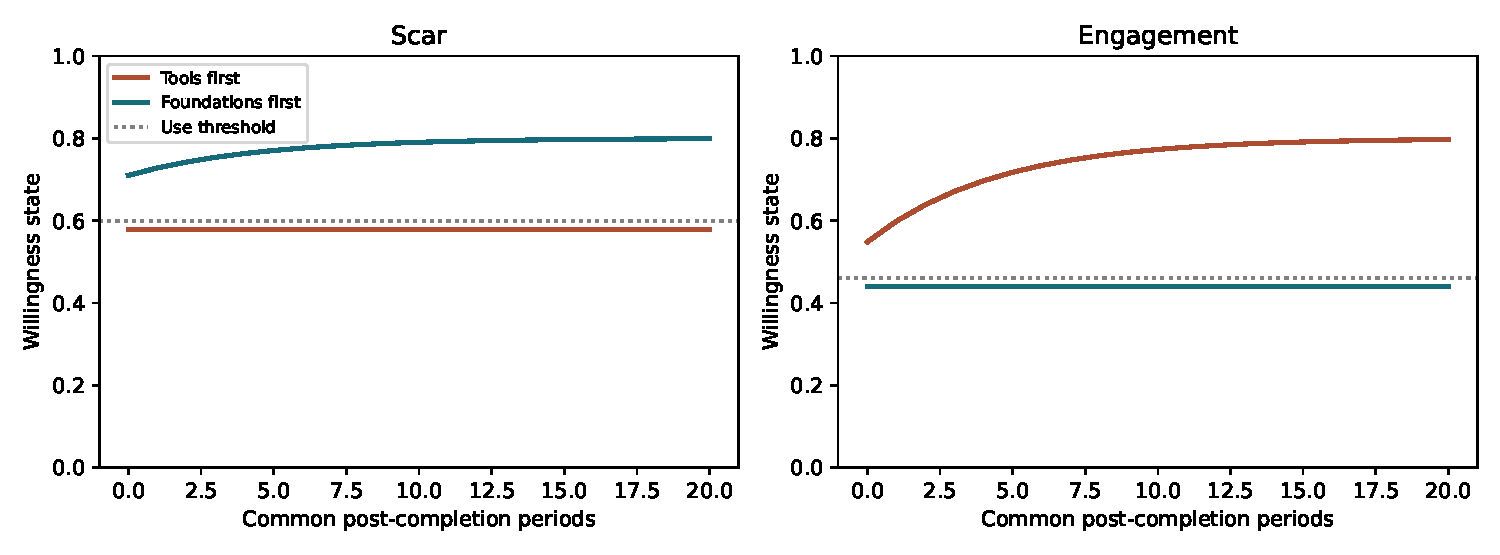
\includegraphics[width=\linewidth]{figures/mechanism.pdf}
\caption{Synthetic willingness trajectories under endogenous feedback. Both resource bundles are complete at period zero in the figure. The dotted line is the use threshold. No field data are shown.}
\end{figure}

With $\beta=.95$, $H=24$, $v=1$, $e=.15$, $b=.05$, and equal installation costs, (\ref{eq:npv}) gives tools-minus-foundations NPV of about $-12.68$ in the scar example and $12.88$ in the engagement example. These values depend on arbitrary surplus units and must not be interpreted as currency or calibrated returns. For the scar state, one validation at $\lambda=.20$ is sufficient: $.8(.578)+.2(.8)=.6224$. The recovery example is especially revealing because a small repair requirement can still entail a long wait when opportunities are rare. Exact outputs appear in the generated tables, which take precedence over rounded text.

\subsection{A design simulation with exposure and carryover}
The simulation is an estimator stress test, separate from the deterministic threshold model. Each experiment randomizes $N$ teams equally. Set $Z=1$ for foundations-first, tool availability $E_{it}=\max(t-4Z_i,0)$ in weeks $t=1,\ldots,16$, and declare the endpoint to be the mean of weeks 13--16 before generating outcomes. Both components are complete before week 9. The synthetic outcome is
\begin{equation}
 Y_{it}=.03t+\gamma(1-e^{-E_{it}/4})
 +Z_i\theta\rho^{\max(t-9,0)}+u_i+\eta_{it},\label{eq:sim}
\end{equation}
where $u_i\sim N(0,.8^2)$ and $\eta$ is stationary Gaussian AR(1) with coefficient $.6$, marginal variance 1, and innovation standard deviation $.8$. All teams are independent. The positive carryover term favors foundations-first; it represents a generic state effect, not an estimate of the trust model.

Four scenarios are predeclared: exact null $(\gamma,\theta)=(0,0)$; duration only $(.6,0)$; transient carryover $(.6,.25,\rho=.65)$; and persistent carryover $(.6,.25,\rho=1)$. Duration alone generates a nonzero policy effect because exposure differs. Calling that effect permanent path dependence would be a category error. The known policy truth is computed directly from (\ref{eq:sim}), not from noisy Monte Carlo estimates.

The valid estimator compares team-level endpoint means with a Welch interval. A deliberately invalid comparator treats all four team-week rows as independent. A second failure case selects complete cases with probability $\operatorname{logit}^{-1}(.9+.5\bar Y_i-.6Z_i)$, thereby making missingness related to both assignment and outcomes. This selection is deliberately nonignorable; no claim is made that inverse probability weighting on baseline covariates repairs it. The full CSV reports bias, empirical standard deviation, average standard error, coverage, rejection of zero, and complete-case bias for every cell. Monte Carlo uncertainty in coverage near .95 is approximately .0049.

\begin{table}[ht]\centering\small
\caption{Synthetic experiments: selected results at 96 independent teams.}
\begin{tabular}{lrrrr}\toprule
Scenario & Truth & Coverage & Power / size & Naive coverage\\\midrule
null & 0.000 & 0.953 & 0.048 & 0.754\\
duration only & -0.029 & 0.952 & 0.050 & 0.731\\
transient carryover & -0.002 & 0.950 & 0.050 & 0.721\\
persistent carryover & 0.221 & 0.951 & 0.169 & 0.736\\
\bottomrule\end{tabular}
\par\smallskip\parbox{.92\linewidth}{\footnotesize Coverage refers to the known policy truth. Power / size is rejection of zero; only the null row measures size. Naive intervals ignore within-team dependence. Each cell uses 2,000 synthetic experiments.}
\end{table}
Repeated measurements increase information about a team's endpoint but do not create additional randomized teams. Precision calculations use the variance of a four-week mean, $.64+[4+2\sum_{k=1}^3(4-k).6^k]/16$. They are planning sensitivities, not power guarantees. Baseline adjustment is omitted from the simulation; a separate table reports the hypothetical reduction if a baseline measure explains 40\% of endpoint variance.

\section{Proposed sequence-policy experiment: not executed}\label{app:protocol}
This appendix is a proposed study only. Its original rollout-policy estimand does not identify the new Bayesian screening-versus-diagnosis decomposition or estimate any structural trust parameter. A separate adaptive policy experiment would need to assign rules permitting no remediation and retain all stopped units; conditioning on completed remediation would select on the policy. The equal-count theoretical comparison fixes assigned diagnostic counts and production dates, whereas the rollout below deliberately includes different access histories. To test the rational mechanism, measure beliefs about final effectiveness before and after physical repair, knowledge of the reset, and the precision, fee and complete disclosure of any public validation. A generic carryover coefficient is not a structural counterpart of these quantities.

\subsection{Setting, unit, policies, and estimands}
The proposed setting is repeated replenishment forecasting at operational teams. This is a concrete design choice, not a recruited organization. The randomization unit is a team with a separate manager, data pipeline, and inventory responsibility. Teams sharing staff, dashboards, or stock allocation should be merged into larger assignment clusters before randomization. Eligible units must have a repeatable manual process, complete baseline logging, and a tool capable of shadow scoring without autonomous execution. Decision authority and remuneration are held fixed by the implementation protocol.

Component $F$ remediates a frozen list of source-field defects, adds validation tests, and supplies documented ownership and freshness checks. Component $A$ integrates the same frozen forecasting engine and interface into the decision workflow, with identical onboarding and recommendation logging. Engine version, permissions, training hours, installation milestones, and accepted field tests are frozen before allocation. Initial quality can differ across teams; baseline blocking records it rather than pretending that remediation has identical realized impact.

Four baseline weeks precede two synchronized four-week implementation phases. In phase 1, foundations-first receives $F$ and tools-first receives $A$ with a scored early demonstration. In phase 2, each receives the other component. Existing components remain available. At the end of phase 2, both receive the same scripted completed-system validation block. Weeks 9--16 form the common observation period; weeks 13--16 are the primary endpoint window. Extended follow-up at weeks 25--28 is separately declared and exploratory unless funded before assignment. There is no simultaneous arm in the primary design.

Each component has the same fixed allocation of implementation hours and purchased services regardless of order. The early tools demonstration is charged to the tools-component allocation; foundations-first receives that same onboarding allocation when its tools arrive. The common completed-system validation block is separately identical in both arms. Opportunity costs of early operating use and differences in realized labor enter the economic ledger even if nominal budgets match. For the baseline model comparison, foundations-first onboarding uses orientation and unscored practice; its only scored system-performance trial before follow-up is the common validation block. If implementation requires an additional scored introductory trial for that arm, freeze and analyze the equal-number-of-trials alternative in Appendix~\ref{app:behavior} instead; the tools-first activation advantage no longer follows. Technical acceptance requires all prespecified critical-field checks to pass in both arms; residual defect rates and uncertainty are reported. A nonsignificant difference in final quality does not prove equivalence. If the same technical bundle is not achieved, the ITT remains a rollout-policy effect including fidelity, but it cannot validate matched-final-resource path dependence.

Let $s=(\text{order},\text{phase dates},\text{assigned intensity},\text{validation schedule})$. The potential outcome $Y_{i,T}(s)$ is the team-level mean operating contribution per eligible baseline-capacity week at the declared endpoint. Contribution subtracts inventory holding, stockout, decision labor, and tool operating costs, using accounting weights frozen before allocation. Fixed rollout costs are excluded from this endpoint and included in NPV. A baseline-capacity denominator prevents selective removal of difficult decisions from mechanically raising measured performance. Team closure receives a prespecified terminal operating value, not an invented zero observation.

The primary estimand is
\begin{equation}
 \Delta_T=E[Y_{i,T}(s_F)-Y_{i,T}(s_T)],\quad T=\text{weeks 13--16}.
\end{equation}
It is the effect of assigning the complete implementation policies, including their different exposure histories. A second estimand reports cumulative transition contribution over weeks 1--8, net of phase-specific costs. A third reports total NPV through week 16 with a prespecified discount rate and a sensitivity grid. These are different economic questions. The sign of a post-completion contrast need not match total project welfare.

For the proposed field study, value resource inputs in baseline-period real currency at frozen hourly and accounting rates. Use an annual real discount rate of 5\%, converted to a weekly factor $(1.05)^{-1/52}$, with 0\% and 10\% annual sensitivities. The model's illustrative $\beta=.95$ has no weekly calibration. The primary NPV stops at week 16; any extrapolation beyond observed follow-up is explicitly modeled, separately labeled, and accompanied by decay and abandonment sensitivities. Cumulative transition welfare is reported undiscounted as well as discounted within NPV.

\subsection{Assignment and analysis}
Randomize 1:1 within blocks defined before allocation by site, baseline defect rate, team size, and baseline outcome. Use blocks of four where possible, with an auditable seed generated after eligibility is locked. The primary analysis is an intention-to-treat team-level ANCOVA with treatment, block effects, and the baseline endpoint. Report the assignment coefficient, confidence interval, and a block-respecting randomization test of the sharp null. Randomization identifies the policy effect under consistency, positivity, and the declared interference restriction; it does not identify the mediator effect. With few clusters, conventional asymptotic cluster intervals are inadequate. The analysis must use the actual assignment scheme, avoid high-dimensional baseline controls, and report uncertainty rather than retrospective power.

There is one confirmatory economic endpoint, tested two-sided at .05. Use, behavioral reliance, decision error, trust survey, and abandonment form a secondary family with Holm adjustment. Transition welfare and NPV are reported as prespecified secondary economic summaries with confidence intervals; claims of significance across the three economic summaries also use Holm correction. Baseline-readiness interaction is prespecified as exploratory, continuous, and tested without searching for a favorable cutoff. A statistically null average does not rule out heterogeneity, but the study is not powered to choose a complex personalized policy.

No actual pilot variance exists. Using the synthetic variance above, $N=96$ yields an approximate unadjusted 80\% minimum detectable effect of .635 synthetic outcome units, or .492 if baseline adjustment truly removes 40\% of variance. The illustrative persistent effect is only about .22; substantially more independent teams would be needed to detect it reliably. Before launch, obtain blinded baseline variance and implementation capacity, define the minimum worthwhile effect in currency, and recalculate. A small single-firm trial should be sold as estimation and feasibility work, not a decisive test of modest organizational gains.

At the synthetic effect of .2214, the normal-approximation requirement is roughly 790 independent teams without baseline adjustment, or 474 if the assumed 40\% variance reduction is realized, before attrition, blocking gains, and multiplicity. Neither count has been secured. The proposed architecture is implementable in principle, but a sufficiently powered field test is not yet demonstrated to be feasible.

\subsection{Exposure accounting and mechanism tests}
Record tool-access hours, recommendations shown, tasks attempted, feedback observed, corrected-field share, staff turnover, training hours, technical downtime, and version changes at team-week level. Availability, receipt, and actual use are separate variables. Nominal budgets are matched, while realized labor and remediation overruns are reported. Equal budgets do not guarantee equal effective treatment.

The primary randomized contrast must not condition on these post-assignment quantities. Plot outcome and use trajectories against calendar time and separately against cumulative scored opportunities as descriptive diagnostics. At matched cumulative exposure, calendar time and composition can differ; those comparisons are not automatically causal. Under the proposed two-arm rollout, availability duration and assignment are closely linked, making an unrestricted regression decomposition unidentified or dependent on functional-form assumptions. Report that limit instead of treating a regression residual as a trust scar.

Mechanism evidence includes choices to request or reject a recommendation on common, incentivized, scored benchmark tasks, stated expected accuracy before the task, and subsequent forecast revisions. Surveys alone are insufficient. A candidate rescue study randomizes an additional fixed block of genuine scored validation to all teams after the primary endpoint, stratifying by original assignment and baseline readiness. Randomizing all teams avoids selecting treatment-dependent nonusers for the main rescue comparison. Estimate the rescue ITT and its interaction with sequence. If targeting nonusers for a separate pilot, interpret its estimand within the observed selected population, not as a comparison of common principal strata.

The rescue is optional and separately budgeted; the original equal-budget sequence estimand ends before it. Extra validation that closes the gap is consistent with an experience mechanism but does not prove psychological trust mediation. Skills, understanding of incentives, and attention may change too. To make a more specific claim, measure these alternatives, keep instructions and incentives identical, and test prespecified exclusion restrictions rather than assume them. Persistence after a finite number of common tasks is evidence of persistence over that experience range, never proof of an infinite-horizon trap.

\subsection{Threats, falsification, and feasibility}
Synchronized phases address common calendar shocks but not arm-specific outages. Log rollout fidelity independently. Spillovers from shared analysts or inventories can attenuate or reverse effects; predefine clusters and report contamination. Retain every randomized unit in the denominator. Separate true zero production from missing accounting records. Report missingness by assignment, baseline predictors, and period. Use transparent bounded-outcome sensitivity intervals with operationally justified bounds, not only a missing-at-random imputation. If bounds are too wide, causal precision is unavailable. A completer analysis is a selection diagnostic, not the headline estimate.

Blind benchmark scoring and freeze cost weights to reduce outcome manipulation. Post-treatment turnover is part of the policy effect, with composition reported. For administrative attrition unrelated to assignment, state and check the assumption before imputation. Interference beyond clusters requires a redesigned saturation or network experiment, not an unannounced no-spillover claim.

The evidence-starvation account is weakened if availability and scored experience remain equal while reported trust alone differs; if measured state fails to predict optional evidence requests on common tasks; if any gap vanishes as exposure saturates; or if a common validation block affects neither reliance nor outcomes despite adequate precision. A persistent resource-quality gap would instead indicate treatment fidelity or technological durability, not a matched-final-bundle sequence effect. Rational rejection of bad recommendations is not an organizational failure.

No suitable authorized panel with assigned sequence, actual use, trust, and dense exposure records was supplied. Census MOPS was checked as a candidate: public tables describe management practices, and detailed linked establishment research requires restricted-data access. It does not provide the randomized sequence or dense mechanism history required here. PITEC is a literature-based candidate for descriptive transition replication, but current access conditions were not verified directly and no files were obtained. Neither is represented as an executable causal substitute. Partner recruitment, data agreements, privacy review, operational feasibility, and a powered cluster count remain prerequisites.

\section{Technical qualifications and extensions}
\subsection{General common-history criterion}
Represent the complete payoff-relevant state by $z$, installation maps by $M_F,M_A$, and a common post-completion transition kernel by $K$. Equality of physical capital does not imply $M_AM_F(z)=M_FM_A(z)$. If the complete terminal states coincide and future policies and shocks share the same law, all future outcome distributions coincide by repeated application of $K$. If $K$ contracts a state distance at rate $\kappa<1$ and payoff is Lipschitz with constant $L$, a coupled expected payoff gap is bounded by $L\kappa^h d(z_T,z_F)$ after $h$ periods. A nonzero limiting gap therefore requires failure of global contraction, different future inputs, or a discontinuous payoff that invalidates the bound. This is a sufficiency argument, not a claim that all path dependence must take our threshold form.

\subsection{Passive recovery and depreciation}
If nonusers' states instead evolve as $x_{h+1}=(1-\delta)x_h+\delta\bar x$, $\delta>0$, then an inactive state converges to $\bar x$. If $\bar x>c$, it crosses $c$ in finite time and the permanent trap disappears. If $\bar x=c$, it approaches from below without crossing in finite time. If $\bar x<c$, nonuse can remain invariant. Depreciation toward a pessimistic reference can also erode active states unless experience offsets it; the invariant-region proof would then need to be redone. Our baseline sets $\delta=0$ and never claims robustness to arbitrary forgetting.

\subsection{Stochastic observations}
Deterministic quality blocks suppress sampling risk. With noisy trials, initial activation probabilities replace indicators in expected NPV. If active feedback can push a state below $c$, active use need no longer be absorbing. Repeated independent successful validations can still yield recovery under appropriate support conditions, but the exact negative-binomial expression no longer applies when bad draws can reverse progress. The numerical illustrations do not establish robustness to this extension. Estimating real recovery requires the distribution of experienced signals, not only their average.

\subsection{Repair choices and the constrained optimum}
If the planner can purchase $n(x)$ guaranteed genuine validation blocks immediately before production, define their total cost $C(x)$, including lost operating time. In a finite horizon, repair is worthwhile when the recovered discounted surplus exceeds $C(x)$. If the blocks are simultaneous and all scored before production, this comparison is $\beta^2vS_H>C(x)$; if they take separate periods, use the truncated discounted activation payoff instead. The best implementation policy in this enlarged menu maximizes each sequence's baseline NPV plus its optimal repair gain. This can reverse a foundations-first recommendation. It is incorrect to call tools-first intrinsically inferior without specifying the feasible rescue technology.

\section{Protocol data dictionary and empty reporting shell}
\small
\begin{longtable}{p{.20\linewidth}p{.19\linewidth}p{.52\linewidth}}
\toprule Field & Unit / timing & Definition and role\\\midrule\endhead
team\_id, block & Team, baseline & Stable pseudonym and randomization block; frozen eligibility roster.\\
assignment & Team, baseline & Original sequence; never overwritten by actual receipt.\\
eligible\_capacity & Team, baseline & Frozen capacity for weekly operating contribution denominator.\\
contribution & Team-week & Revenue less prespecified variable, inventory, stockout, labor, and operating costs.\\
rollout\_cost & Team-week & Installation, remediation, training, downtime and validation resource cost; NPV input.\\
quality\_score & Team-week & Frozen field-test pass rate and freshness; not a success-based data-driven index.\\
tool\_hours & Team-week & Availability from logs, including planned and unplanned downtime.\\
shown, attempted & Team-week & Eligible recommendations displayed and tasks attempted; retain denominators.\\
feedback\_count & Team-week & Scored outcomes actually seen, distinguished from recommendations merely displayed.\\
reliance & Common task & Incentivized recommendation request, weight or choice; behavior, not survey trust.\\
expected\_accuracy & Before common task & Elicited prediction of tool accuracy, with scoring incentives if feasible.\\
trust\_survey & Baseline and phase ends & Prespecified repeated scale; secondary and subject to reporting error.\\
error\_loss & Common task & Blinded benchmark loss with a fixed scoring rule; decision quality measure.\\
abandonment & Team-week & Zero voluntary use over two consecutive eligible weeks; distinct from no access.\\
staff, training & Team-week & Roster changes and hours by role; implementation and composition checks.\\
missing\_reason & Every endpoint & Distinguish unrecorded accounts, closure, transfer, refusal, and true zero.\\
rescue\_assignment & Team, after week 16 & Optional independent validation allocation; separate from main policy.\\
\bottomrule
\end{longtable}
\normalsize
\begin{center}
\begin{tabular}{p{.40\linewidth}p{.22\linewidth}p{.22\linewidth}}
\toprule Proposed field result & Effect estimate & Confidence interval\\\midrule
Weeks 13--16 contribution ITT & Not collected & Not collected\\
Weeks 1--8 transition welfare & Not collected & Not collected\\
Total NPV through week 16 & Not collected & Not collected\\
Behavioral reliance & Not collected & Not collected\\
Optional validation ITT & Not collected & Not collected\\\bottomrule
\end{tabular}
\end{center}
No empirical cell is populated with a synthetic result.

\section{Exact cost-region reproduction certificate}\label{app:costcertificate}
The analytical partition is proved in Section~\ref{sec:regions}; the executable check is \texttt{code/cost\_regions.py}. It uses Python's exact rational arithmetic rather than a floating-point policy grid. For each declared fee/reset slice it constructs the affine cost boundaries, enumerates their intersections and one representative per intervening interval, and compares the analytical strict and weak predicates with the original menu values. The run checks 20,224 baseline cost cases and 4,996 cases for additional primitives, including an uninformative early diagnostic and a diagnostic outside the dominance premise for the unrestricted weak table. Eight exact corners check the open positive-region witness, and 240 cases check reset contraction. All passed. These finite checks supplement the continuous-parameter proofs; they are not a numerical proof covering all real likelihoods or reset values.

The file \texttt{output/cost\_region\_verification.json} records actual counts and the exact reset witness $838/1235$. The five baseline fee cells are exported in \texttt{certificate\_fee\_partition.csv}. Older grid and synthetic inference outputs remain supplementary. The reproduction shell script regenerates all results and PDFs and fails on assertions or compilation errors. The author critical audit is identified as such and does not substitute for independent scientific review. Every empirical reporting cell in Appendix F remains unfilled because no proposed study has been run.

\end{document}
